\section{Metodología}

Se estudiará el comportamiento de cada etapa por separado del circuito base, el circuito completo, la respuesta en frecuencia, al circuito realimentado.

\begin{ilustracion}[ht]
    \centering
    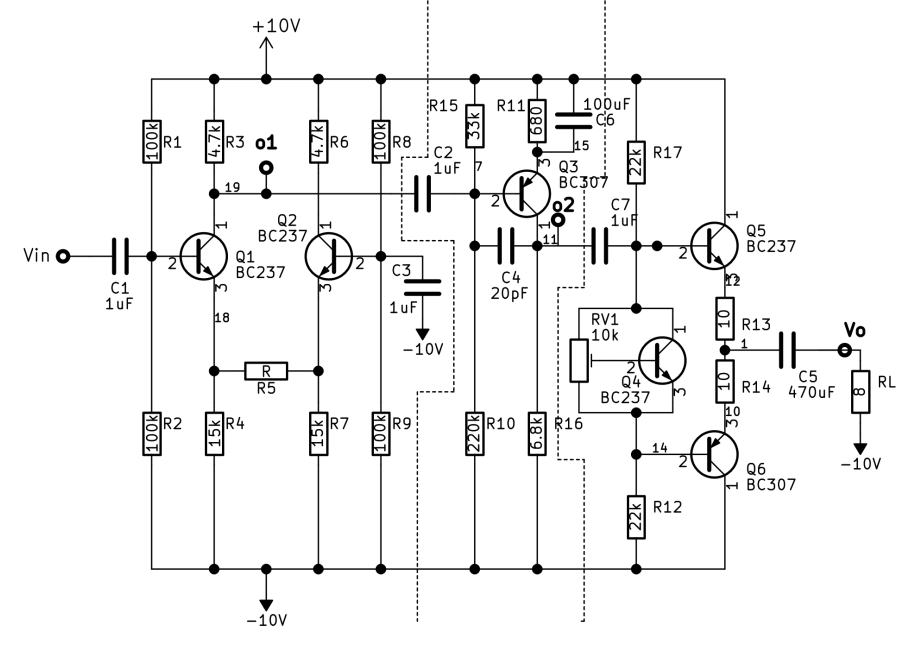
\includegraphics[width=0.9\textwidth]{src/images/metodología/circuito-base.png}
    \caption{Circuito base}
    \label{ilus:met-circuito-base}
\end{ilustracion}
    
\subsection{Amplificador de potencia}

En primer lugar identificamos la etapa del amplificador de potencias en el diagrama del amplificador multietapas, la cual es la que contiene a los transistores $Q4$, $Q5$ y $Q6$. Dicha etapa se muestra en la ilustración \ref{ilus:met-etapa-amplificador-de-potencia}.

\begin{ilustracion}[ht]
    \centering
    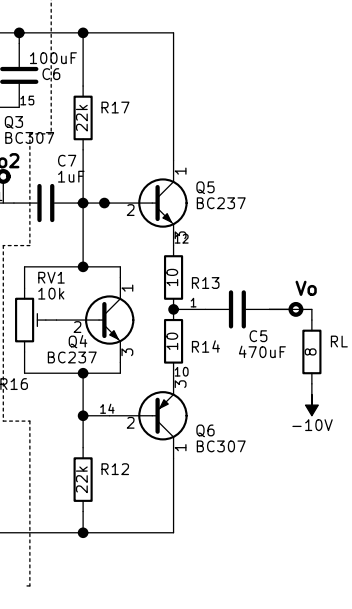
\includegraphics[width=0.23\textwidth]{src/images/metodología/etapa-de-potencia.png}
    \caption{Etapa del amplificador de potencia}
    \label{ilus:met-etapa-amplificador-de-potencia}
\end{ilustracion}

Ahora procedemos a calcular los puntos estáticos de operación, para ello tomamos los capacitores como circuitos abiertos, ya que estamos trabajando en DC y empezamos a calcular las corrientes en el transistor $Q4$.

Asumiremos que las corrientes de base $I_{bQ5}$ e $I_{bQ6}$ son muy pequeñas en comparación con la corriente $I_{R17}$ por tanto la tomaremos como despreciables.

Ahora aplicando LCK en el multiplicador de voltaje ($Q_4$):
\begin{equation}
I_{RV1} + I_{cQ4} = I_{R17}    
\end{equation}

Si ahora asumimos $I_bQ4$ despreciable:

\begin{equation}
    I_{RV1} = \frac{V_{BEQ4}}{XR_{V1}}
\end{equation}

Aplicando LVK tenemos:

\begin{equation}
    V_{CEQ4} = I_{RV1} * R_v1
\end{equation}

Usando (2) y (3):

$$ V_{CEQ4} = \frac{V_{BEQ4}}{X*R_{V1}} * R_{V!}$$

\begin{equation}
    V_{CEQ4} = \frac{V_{BEQ4}}{X}
\end{equation}

Debido a que el amplificador es de clase AB el voltaje $V_{CEQ4}$ tiene que ser dos veces el voltaje base emisor $V_{be}$ para los transistores $Q5$ y $Q6$ estén lo más cerca posible de la zona activa y se pueda reducir el efecto crossover de la salida.

Aplicando LVK entre las dos referencias tenemos:

$$10V - R_{17}*I_{17} - 2V_{beQ4} - R_{12}*I_{17} + 10V = 0$$

despejando $I_{17}$:

\begin{equation}
    I_{17} = \frac{20 - 2V_{beQ4}}{R_{17} + R_{12}}
\end{equation}

Usando (1), (2) y (5) tenemos:

\begin{equation}
    I_{cQ4} = \frac{20 - 2V_{beQ4}}{R_{17} + R_{12}} - \frac{2V_{beQ4}}{R_{V1}}
    \label{eq:icQ4}
\end{equation}

Usando la ecuacion (\ref{eq:icQ4}) y los datos:

$V_{beQ4} = 0.62 V$ 

$R_{17} = R_{12} = 22k\Omega$ :

$R_{V1} = 10k\Omega$ 

$$    I_{cQ4} = \frac{20 - 2 * 0.62 V}{22k\Omega + 22k\Omega} - \frac{2 * 0.62 V}{10 k\Omega} $$

$$ I_{cQ4} = 302.36 \mu A$$

Tomando $hfe_{Q4} = 230$

\begin{equation}
    I_{bQ4} = I_{cQ4} / hfe
\end{equation}

$$ I_{bQ4} = 1.31 \mu A$$

$$ V_{ceQ4} = 2 * 0.62 V = 1.24 V$$

Ahora, volviendo a despreciar las corriente de base y aplicando LVK en la malla con los transistores

$$V_{ceQ4} - V_{beQ5} - I_{eQ5}* (R_{13} + R_{14}) - V_{beQ6} = 0$$

despejando $I_{eQ5}$

\begin{equation}
    I_{eQ5} =\frac{ V_{ceQ4} - V_{beQ5} - V_{beQ6} }{R_{13} + R_{14}}
\end{equation}

Tomando $V_{beQ5} = V_{beQ4} = 0.62 V$ y $V_{beQ6} = 0.55 V$, entonces: 

$$I_{eQ5} = \frac{ 1.24 V - 0.62 V - 0.55 V }{10 \Omega + 10 \Omega }$$

$$ I_{eQ5} = I_{eQ6} \approx I_{cQ5} \approx I_{cQ6} = 350\mu A$$

Basado en las I de emisor ahora calulamos las corrientes de base, asumiendo que $hfe_{Q5} = 230 $ y $hfe_{Q6} = 150$

$$I_{bQ5} = I_{cQ5} / hfe = 350\mu A / 230 = 1.52 \mu A $$

$$I_{bQ6} = I_{cQ6} / hfe = 350\mu A / 150 = 2.33 \mu A $$

Se asume que $V_{ceQ5} = V_{ceQ6} $, por tanto:

$$ 10 - 2 V_{ceQ5} - (R_{14} + R_{13}) * I_{eQ5} + 10 = 0$$

despejando $V_{ceQ5}$ tenemos:

\begin{equation}
    V_{ceQ5} = V_{ceQ6} = \frac{ 20 - (R_{14} + R_{13}) * I_{eQ5} }{2}
\end{equation}

por tanto 

$$ V_{ceQ5} = V_{ceQ6} = \frac{ 20 V - (10 + 10) \Omega * 350\mu A }{2} = 9.99 V$$

El resumén de los puntos estáticos de operación del amplificador de potencia se muestran en la tabla \ref{tab:amplificador-de-potencia-puntos-estaticos}.

\begin{table}[ht]
    \centering
    \begin{tabular}{|c|c|c|}
        \hline
        Transistor & \textbf{$I_c$} & \textbf{$V_{ce}$} \\
        \hline
        $Q4$ & $302.36 \mu A$ & $1.24 V$ \\
        $Q5$ & $350\mu A$ & $9.99 V$ \\
        $Q6$ & $350\mu A$ & $9.99 V$ \\
        \hline
    \end{tabular}
    \caption{Puntos estáticos de operación del amplificador de potencia}
    \label{tab:amplificador-de-potencia-puntos-estaticos}
\end{table}

A continuación, en la ilustración \ref{ilus:met-puntos-estaticos-amplificador-de-potencia} se muestran los puntos estáticos de operación del amplificador de potencia.

\begin{ilustracion}[ht]
    \centering
    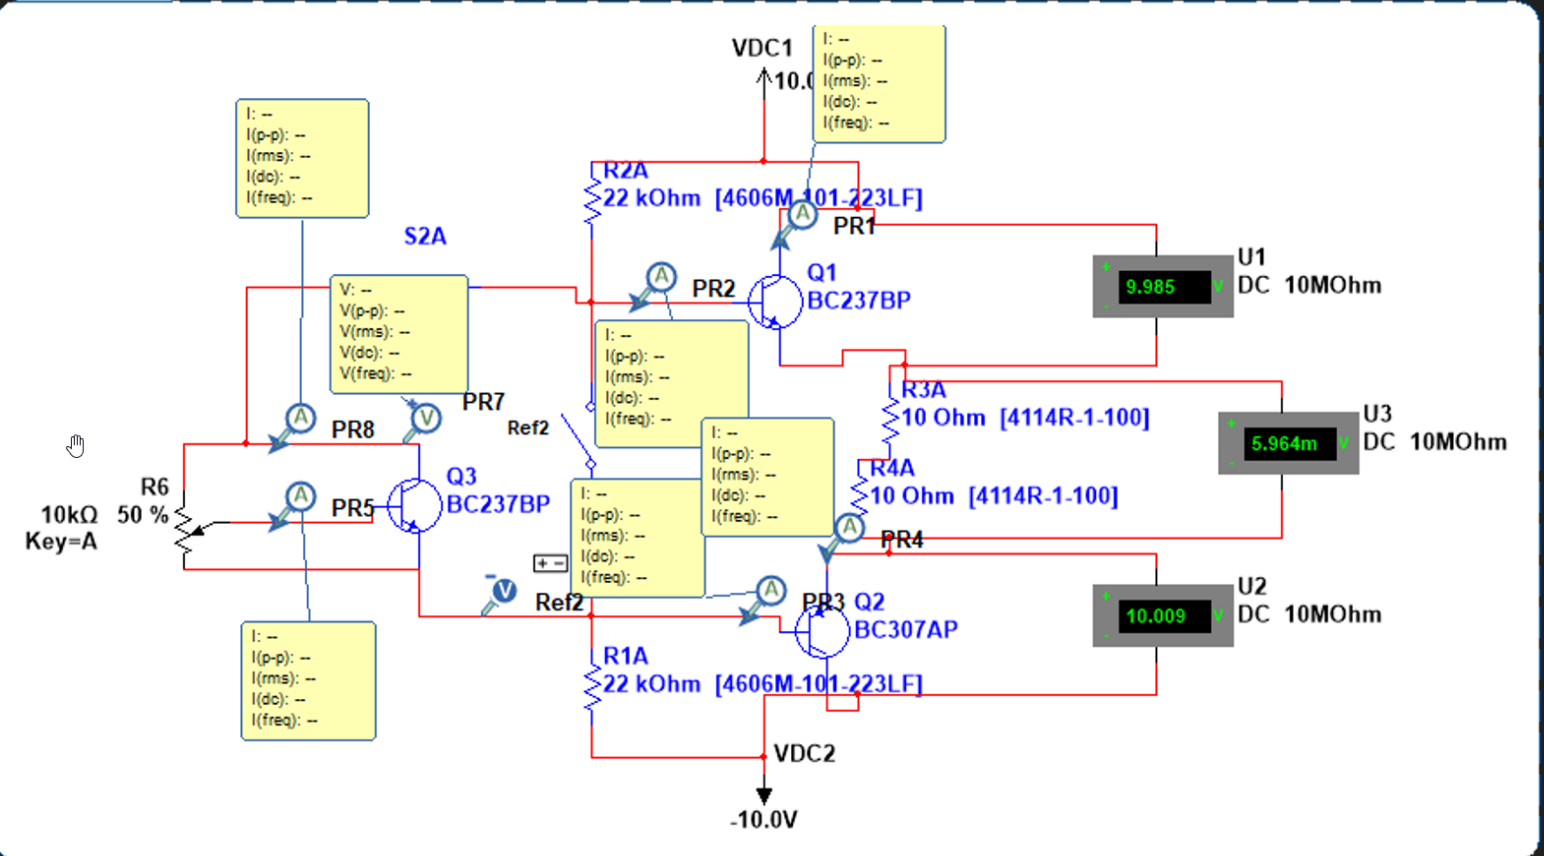
\includegraphics[width=0.9\textwidth]{src/images/metodología/simulacion-etapa-potencia-puntos-estaticos.png}
    \caption{Puntos estáticos de operación del amplificador de potencia}
    \label{ilus:met-puntos-estaticos-amplificador-de-potencia}
\end{ilustracion}

Ahora, para la parte dinámica, calculamos los parámetros del transistor utilizando $V_t = 26 mV$ y $V_A = 100 V$

$$gm = \frac{I_c}{V_t} = \frac{0,35 mA}{26 mV}$$

$$gm = 13.46 mS$$

$$R_\pi = \frac{\beta}{gm} = \frac{230}{13.46\times 10^{-3}}$$

$$ R_\pi = 17.07k \Omega$$

$$ R_o = \frac{V_A}{I_c} = \frac{100 V}{0,35 mA} = 285,71 k\Omega$$

Obtenidos los parámetros dinámicos podemos calcular la ganancia del amplificador hacinedo un análisis de las corrientes de entrada y salida del circuito, obteniendo la expresión:

 $$ A = \frac{(1 + gmr_{\pi5})(r_{13} + r_l)r_L}{[r_{\pi 5} + (1 + gmr\pi5)(r_{13} + r_L)](r_{13} + r_L)}$$

 $$A = 0.96 $$

 Ahora, para calcular la impedancia de entrada:

 $$ Z_i = r_{17} \parallel r{12} \parallel [r_{\pi5} + (1 + gmr_{\pi 5})(r_{13} + r_l)] $$
 
 $$ Z_i = 10.77K\Omega $$

 Mientras que la impedancia de salida viene dada por la expresión:

$$ Z_o = r_{13} + \frac{r_{\pi5} + r_{17}/2}{1 + gmr_{\pi5}} $$

 $$ Z_o = 132 \Omega$$

 El modelo dinámico del amplificador de potencia se muestra en la tabla \ref{tab:met-amp-potencia-modelo-dinamico}.

\begin{table}[ht]
    \centering
    \begin{tabular}{|c|c|}
        \hline
        parámetro & valor  \\
        \hline
        $Z_i$ & $10.77k\Omega$ \\
        \hline
        $Z_o$ & $132\Omega$ \\
        \hline
        $A$ & $0.96$ \\
        \hline
    \end{tabular}
    \caption{Modelo dinámico del amplificador de potencia}
    \label{tab:met-amp-potencia-modelo-dinamico}
\end{table}

en la ilustración \ref{ilus:sim-amp-potencia-ganancia} se muestra la ganancia del amplificador de potencia. Se puede observar que el voltaje de entrada y de salida se superponen, ya que la ganancia es aproximadamente 1.

\begin{ilustracion}[ht]
    \centering
    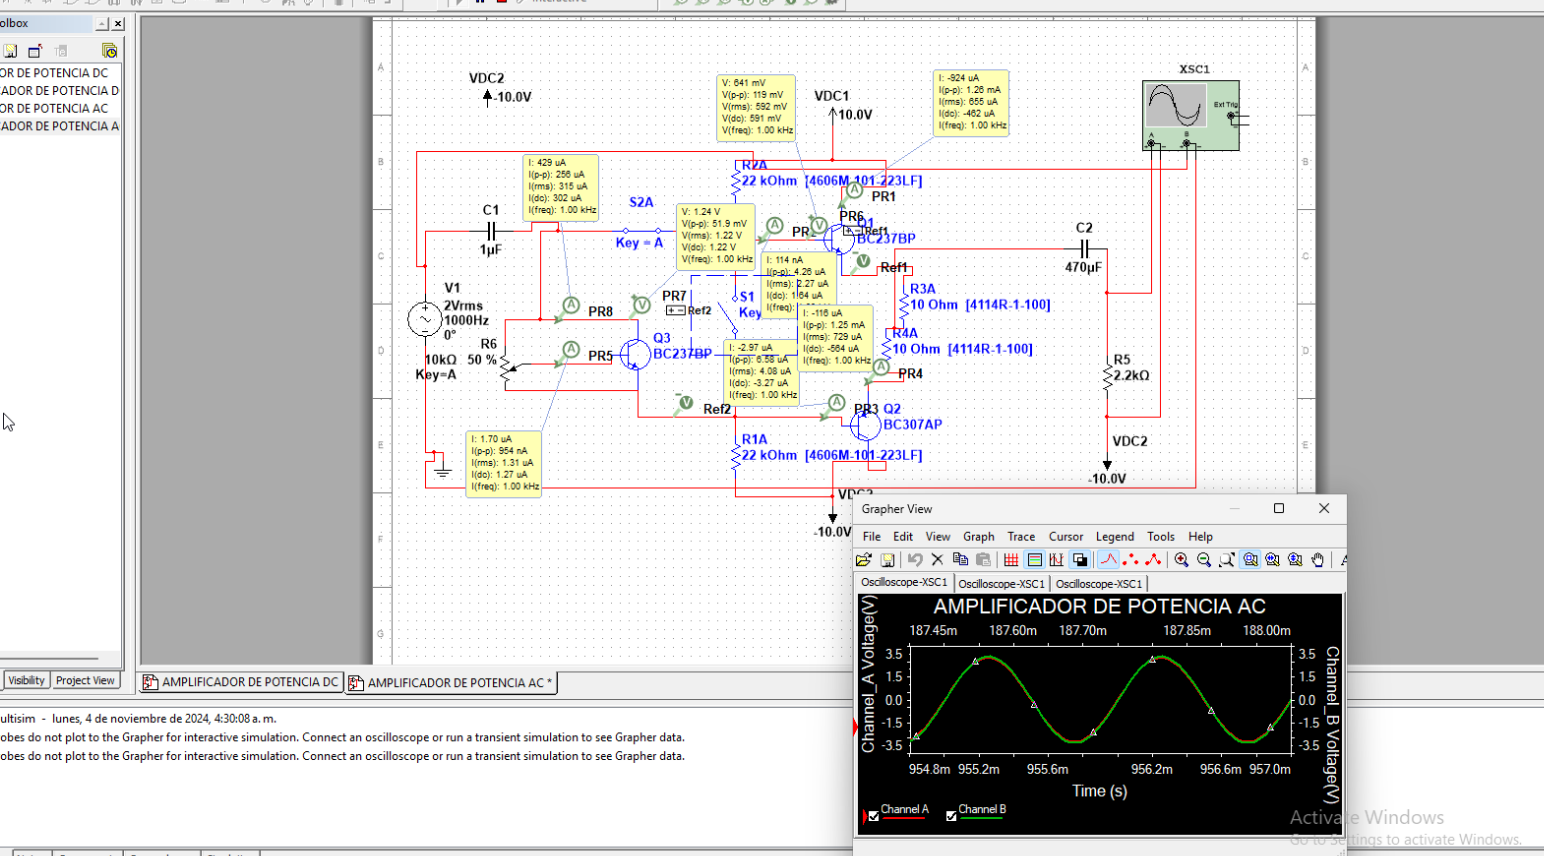
\includegraphics[width=0.9\textwidth]{src/images/p1/p1-sim-ganancia.png}
    \caption{Ganancia del amplificador de potencia}
    \label{ilus:sim-amp-potencia-ganancia}
\end{ilustracion}

En la ilustración \ref{ilus:sim-amp-potencia-efecto-crossover} se muestra el efecto crossover del amplificador de potencia. 

\begin{ilustracion}[ht]
    \centering
    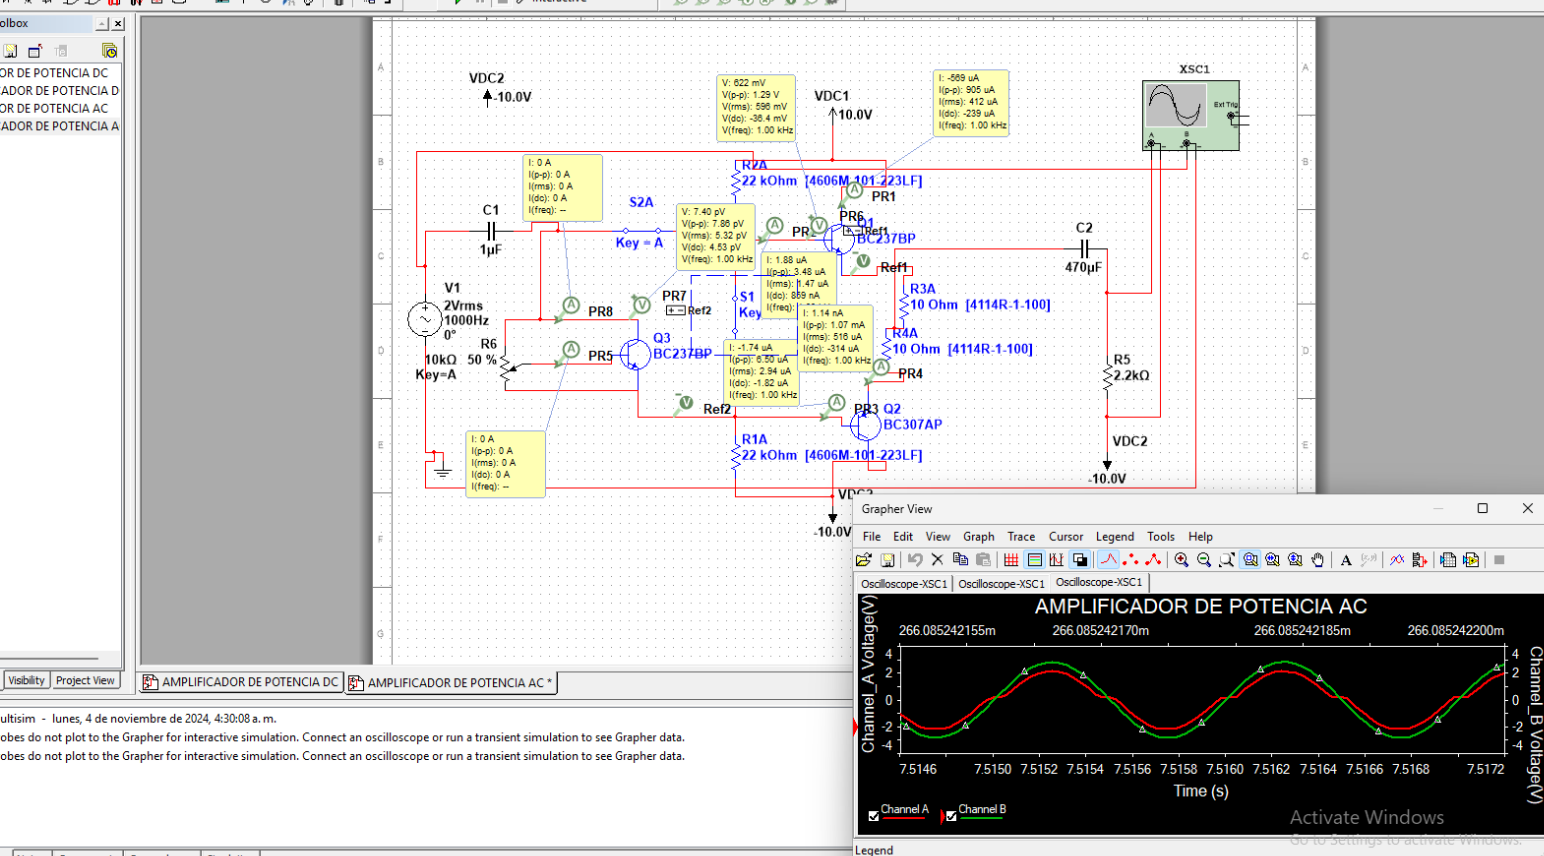
\includegraphics[width=0.9\textwidth]{src/images/p1/p1-sim-efecto-crossover.png}
    \caption{Efecto crossover del amplificador de potencia}
    \label{ilus:sim-amp-potencia-efecto-crossover}
\end{ilustracion}
\FloatBarrier
\subsection{Práctica 2}

\subsubsection{Puntos estáticos de operación etapa diferencial}

El cuadro \ref{tab:med-dc-etapa-diferencial} muestra las mediciones de voltaje DC de los transistores $Q_1$ y $Q_2$ de la etapa diferencial de la práctica 2.

\begin{table}[h!]
\centering
\begin{tabular}{|c|c|c|c|c|c|c|c|c|}
\hline
\textbf{Transistor} & \textbf{\(Vc[V]\)} & \textbf{\(\varDelta Vc[V]\)} & \textbf{\(Vb[V]\)} & \textbf{\(\varDelta Vb[V]\)} & \textbf{\(Ve[V]\)} & \textbf{\(\varDelta Ve[V]\)} & \textbf{\(Rc[\Omega]\)} & \textbf{\(\varDelta Rc[\Omega]\)} \\ \hline
Q1 & 7.2 & 0.2 & -0.016 & 0.002 & -0.6 & 0.04 & 4700 & 235 \\ \hline
Q2 & 7.2 & 0.2 & -0.052 & 0.004 & -0.6 & 0.04 & 4700 & 235 \\ \hline
\end{tabular}
\caption{Mediciones voltaje DC etapa diferencial}
\label{tab:med-dc-etapa-diferencial}
\end{table}

Utilizando los datos en el cuadro \ref{tab:med-dc-etapa-diferencial}, se hayaron las mediciones indirectas de los puntos de reposo de la etapa diferencial, los cuales se muestran en el cuadro \ref{tab:med-puntos-reposo-etapa-diferencial}.

\begin{table}[h!]
\centering
\begin{tabular}{|c|c|c|c|c|c|c|}
\hline
\textbf{Parámetro} & \textbf{Transistor} & \textbf{Valor Teórico} & \textbf{Medición} & \textbf{Incertidumbre} & \textbf{Error Absoluto} & \textbf{Error Relativo} \\ \hline
$I_{c}$ & Q1 & 0.00062 & 0.000595745 & 0.000219015 & 0.00002426 & 3.91\% \\ \hline
$I_{c}$ & Q2 & 0.00062 & 0.000595745 & 0.000219015 & 0.00002426 & 3.91\% \\ \hline
$V_{ce}$ & Q1 & 7.79 & 7.8 & 0.203960781 & 0.01000000 & 0.13\% \\ \hline
$V_{ce}$ & Q2 & 7.79 & 7.8 & 0.203960781 & 0.01000000 & 0.13\% \\ \hline
\end{tabular}
\caption{Mediciones puntos de reposo etapa diferencial}
\label{tab:med-puntos-reposo-etapa-diferencial}
\end{table}

\subsubsection{Modelo dinámico etapa diferencial modo diferencial}

\begin{table}[h!]
\centering
\begin{tabular}{|c|c|c|c|c|c|}
\hline
\textbf{\(Vg[V]\)} & \textbf{\(\varDelta Vg[V]\)} & \textbf{\(Vi[V]\)} & \textbf{\(\varDelta Vi[V]\)} & \textbf{\(Rp[\Omega]\)} & \textbf{\(\varDelta Rp[\Omega]\)} \\ \hline
1.04 & 0.04 & 0.48 & 0.02 & 48000 & 4800 \\ \hline
\end{tabular}
\caption{Impedancia de entrada etapa diferencial modo diferencial}
\label{tab:med-impedancia-entrada-etapa-diferencial modo diferencial}
\end{table}

\begin{table}[h!]
\centering
\begin{tabular}{|c|c|c|c|c|c|}
\hline
\textbf{\(Vo_{sc}[V]\)} & \textbf{\(\varDelta Vo_{sc}[V]\)} & \textbf{\(Vo_{cc}[V]\)} & \textbf{\(\varDelta Vo_{cc}[V]\)} & \textbf{\(Rp[\Omega]\)} & \textbf{\(\varDelta Rp[\Omega]\)} \\ \hline
3.2 & 0.1 & 1.6 & 0.04 & 4700 & 470 \\ \hline
\end{tabular}
\caption{Impedancia de entrada etapa diferencial}
\label{tab:med-impedancia-entrada-etapa-diferencial}
\end{table}

\begin{table}[h!]
\centering
\begin{tabular}{|c|c|c|c|}
\hline
\textbf{\(Vi[V]\)} & \textbf{\(\varDelta Vi[V]\)} & \textbf{\(Vo[V]\)} & \textbf{\(\varDelta Vo[V]\)} \\ \hline
1 & 0.1 & 3.2 & 0.1 \\ \hline
\end{tabular}
\caption{Voltajes de entrada y de salida etapa diferencial modo diferencial}
\label{tab:med-voltaje-entrada-salida-etapa-diferencial}
\end{table}

\begin{table}[h!]
\centering
\begin{tabular}{|c|c|c|c|c|c|}
\hline
\textbf{Parámetro} & \textbf{Valor} & \textbf{Medición} & \textbf{Incertidumbre} & \textbf{Error Absoluto} & \textbf{Error Relativo} \\ \hline
$[Z] i$ & 43990 & 41142.85714 & 5974.907966 & 2847.142857 & 6.47\% \\ \hline
$[Z] o$ & 4700 & 4700 & 602.0083575 & 0 & 0.00\% \\ \hline
$[A]$ & -2.96 & -3.2 & 0.335261092 & 0.24 & 8.11\% \\ \hline
\end{tabular}
\caption{Modelo dinámico etapa diferencial modo diferencial}
\label{tab:med-modelo-dinamico-etapa-diferencial-modo-diferencial}
\end{table}

\begin{figure}[ht]
    \centering
    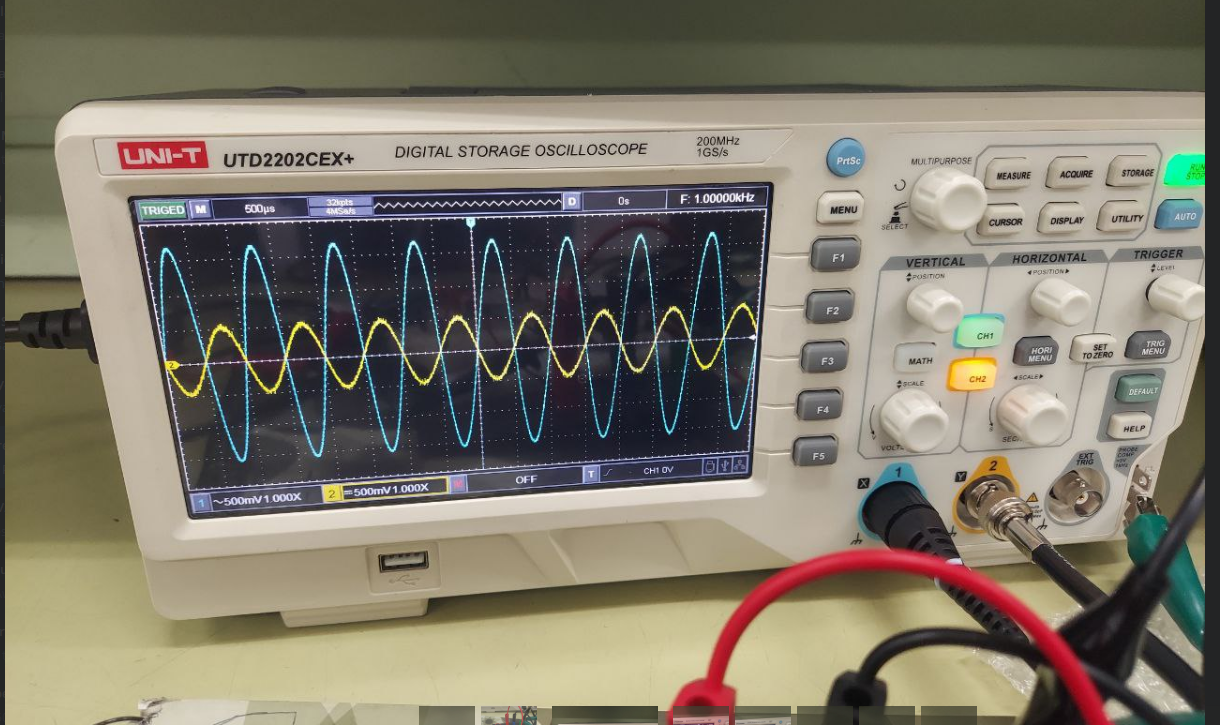
\includegraphics[width=1.0\textwidth]{src/images/resultados/p2/med-ganancia-mod-diff.png}
    \caption{Ganancia etapa diferencial modo diferencial}
    \label{fig:ganancia-etapa-diff-mod-diff}
    
\end{figure}

La máxima excursión de la etapa diferencial se alcanza cuando se pasa el límite de $3 \pm 0.2 V$ en el voltaje de salida $V_o$ en el cuando el voltaje de entrada es $V_i = 1 \pm 0.1 V$.



\subsubsection{modelo dinámico etapa diferencial modo común}

\begin{table}[h!]
\centering
\begin{tabular}{|c|c|c|c|c|c|}
\hline
\textbf{\(Vg[V]\)} & \textbf{\(\varDelta Vg[V]\)} & \textbf{\(Vi[V]\)} & \textbf{\(\varDelta Vi[V]\)} & \textbf{\(Rp[\Omega]\)} & \textbf{\(\varDelta Rp[\Omega]\)} \\ \hline
1.04 & 0.04 & 0.31 & 0.015 & 48000 & 4800 \\ \hline
\end{tabular}
\caption{Impedancia de entrada etapa diferencial modo común}
\label{tab:med-impedancia-entrada-etapa-diferencial-modo-comun}
\end{table}

\begin{table}[h!] \centering \begin{tabular}{|c|c|c|c|} \hline \textbf{\(Vi[V]\)} & \textbf{\(\varDelta Vi[V]\)} & \textbf{\(Vo[V]\)} & \textbf{\(\varDelta Vo[V]\)} \\ \hline 1 & 0.04 & 0.3 & 0.01 \\ \hline \end{tabular} \caption{Voltajes de entrada y salida etapa diferencial modo común} \label{tab:med-voltajes-entrada-salida-etapa-diferencial-modo-comun} \end{table}

\begin{table}[h!]
\centering
\begin{tabular}{|c|c|c|c|c|c|}
\hline
\textbf{Parámetro} & \textbf{Valor} & \textbf{Medición} & \textbf{Incertidumbre} & \textbf{Error Absoluto} & \textbf{Error Relativo} \\ \hline
$Z_i [\Omega]$ & 24500 & 20383.56164 & 2716.026753 & 4116.438356 & 16.80\% \\ \hline
$Z_o [\Omega]$ & 4700 & 4700 & 602.0083575 & 0 & 0.00\% \\ \hline
$A$ & 0.31 & 0.3 & 0.015620499 & 0.01 & 3.23\% \\ \hline
\end{tabular}
\caption{Modelo dinámico etapa diferencial modo común}
\label{tab:med-modelo-dinamico-etapa-diferencial-modo-comun}
\end{table}


\begin{figure}[ht]
    \centering
    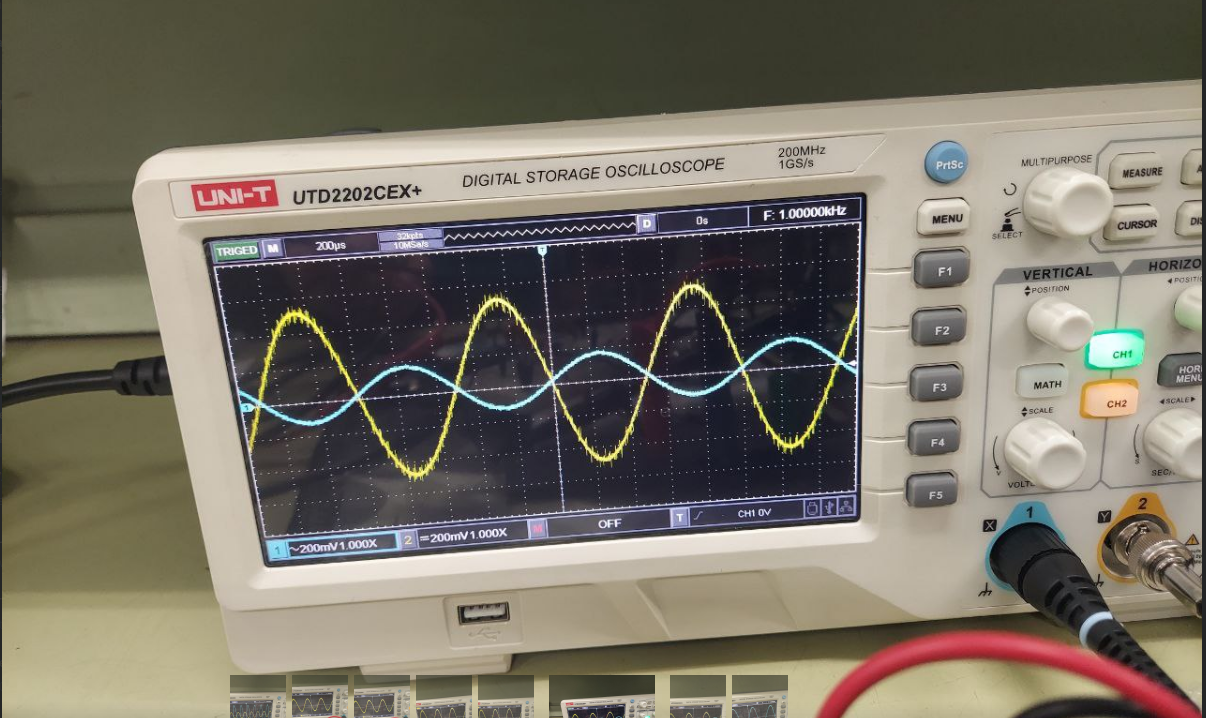
\includegraphics[width=1.0\textwidth]{src/images/resultados/p2/med-ganancia-mod-comun.png}
    \caption{Ganancia etapa diferencial modo común}
    \label{fig:ganancia-etapa-diff-mod-comun}
\end{figure}

% máxima excursion modo diff
\begin{figure}[ht]
    \centering
    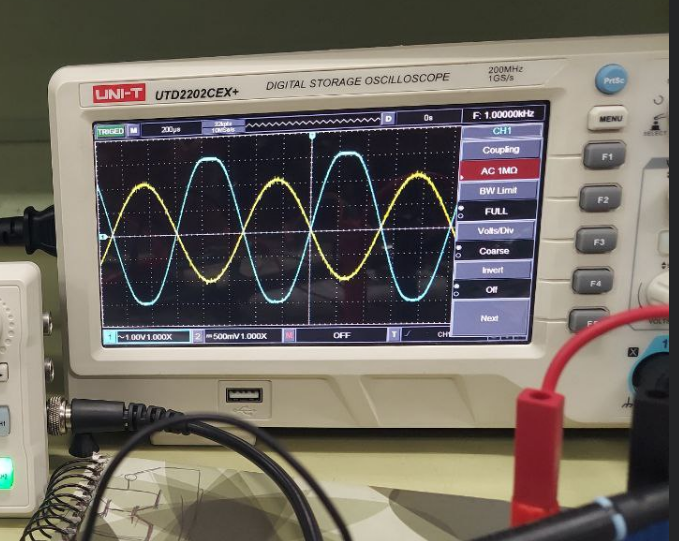
\includegraphics[width=1.0\textwidth]{src/images/resultados/p2/med-maxima-excursion-mod-diff.png}
    \caption{Máxima excursión etapa diferencial modo diferencial}
    \label{fig:max-excursion-mod-diff}
\end{figure}

\FloatBarrier
\subsection{Práctica 3}

\subsubsection{Puntos de operación amplificador multietapas desacoplado}

\begin{table}[h!]
\centering
\begin{tabular}{|c|c|c|c|c|c|c|c|c|c|}
\hline
\textbf{Transistor} & \textbf{\(Vc[V]\)} & \textbf{\(\varDelta Vc[V]\)} & \textbf{\(Vb[V]\)} & \textbf{\(\varDelta Vb[V]\)} & \textbf{\(Ve[V]\)} & \textbf{\(\varDelta Ve[V]\)} & \textbf{\(Re[\Omega]\)} & \textbf{\(\varDelta Re[\Omega]\)} \\ \hline
Q1 & 7.2 & 0.4 & -0.04 & 0.002 & -0.6 & 0.04 & 4700 & 470 \\ \hline
Q2 & 7.6 & 0.4 & -0.068 & 0.004 & -0.64 & 0.04 & 4700 & 470 \\ \hline
Q3 & 8 & 0.4 & 8 & 1 & 7.4 & 0.4 & 6800 & 680 \\ \hline
Q4 & 0.68 & 0.04 & -0.6 & 0.04 & -0.6 & 0.04 & 5000 & 500 \\ \hline
Q5 & 10 & 1 & 0.68 & 0.04 & 0.2 & 0.01 & 20 & 1 \\ \hline
Q6 & -10 & 1 & -0.56 & 0.04 & -0.2 & 0.01 & 20 & 1 \\ \hline
\end{tabular}
\caption{Mediciones voltaje DC de los transistores en el multietapas desacoplado}
\label{tab:med-voltaje-dc-transistores-multietapas-desacoplado}
\end{table}

\begin{table}[h!]
\centering
\begin{tabular}{|c|c|c|c|c|c|c|}
\hline
\textbf{Parámetro} & \textbf{Transistor} & \textbf{Valor Teórico} & \textbf{Medición} & \textbf{Incertidumbre} & \textbf{Error Absoluto} & \textbf{Error Relativo} \\ \hline
$I_{c}$ & Q1 & 0.00062 & 0.000595745 & 0.000236773 & 0.00002426 & 3.91\% \\ \hline
$I_{c}$ & Q2 & 0.00062 & 0.000510638 & 0.000234776 & 0.00010936 & 17.64\% \\ \hline
$I_{c}$ & Q3 & -0.00237 & -0.002647059 & 0.000308473 & 0.00027706 & 11.69\% \\ \hline
$I_{c}$ & Q4 & $0.30\times10^{-04}$ & 0 & 1.13137E-05 & 0.00030236 & 100.00\% \\ \hline
$I_{c}$ & Q5 & $0.35\times10^{-03}$ & 0.02 & 0.001224745 & 0.01965000 & 5614.29\% \\ \hline
$I_{c}$ & Q6 & $0.35\times10^{-03}$ & -0.02 & 0.001224745 & 0.02035000 & 5814.29\% \\ \hline
$V_{ce}$ & Q1 & 7.79 & 7.8 & 0.401995025 & 0.01000000 & 0.13\% \\ \hline
$V_{ce}$ & Q2 & 7.79 & 8.24 & 0.401995025 & 0.45000000 & 5.78\% \\ \hline
$V_{ce}$ & Q3 & 2.27 & 0.6 & 0.565685425 & 1.67000000 & 73.57\% \\ \hline
$V_{ce}$ & Q4 & 1.24 & 1.28 & 0.056568542 & 0.04000000 & 3.23\% \\ \hline
$V_{ce}$ & Q5 & 9.99 & 9.8 & 1.000049999 & 0.19000000 & 1.90\% \\ \hline
$V_{ce}$ & Q6 & -9.99 & -9.8 & 1.000049999 & 0.19000000 & 1.90\% \\ \hline
\end{tabular}
\caption{Puntos estáticos de operación transistor multietapas desacoplado}
\label{tab:med-puntos-estaticos-operacion-transistor-multietapas-desacoplado}
\end{table}

\FloatBarrier
\subsubsection{modelo dinámico etapa impulsora}

\begin{table}[h!]
\centering
\begin{tabular}{|c|c|c|c|}
\hline
\textbf{\(Vi[V]\)} & \textbf{\(\varDelta Vi[V]\)} & \textbf{\(Vo[V]\)} & \textbf{\(\varDelta Vo[V]\)} \\ \hline
0.48 & 0.04 & 10 & 1 \\ \hline
\end{tabular}
\caption{Ganancia etapa impulsora}
\label{tab:med-ganancia-etapa-impulsora}
\end{table}

\begin{table}[h!]
\centering
\begin{tabular}{|c|c|c|c|c|c|}
\hline
\textbf{Parámetro} & \textbf{Valor} & \textbf{Medición} & \textbf{Incertidumbre} & \textbf{Error Absoluto} & \textbf{Error Relativo} \\ \hline
$[Z] i$ & 2310 & & & & \\ \hline
$[Z] o$ & 6800 & & & & \\ \hline
$[A]$ & 619.9 & 20.8333333333333 & 2.711892249 & 599.0666667 & 96.64\% \\ \hline
\end{tabular}
\caption{Modelo dinámico etapa impulsora}
\label{tab:med-modelo-dinamico-etapa-impulsora}
\end{table}

\begin{figure}
    \centering
    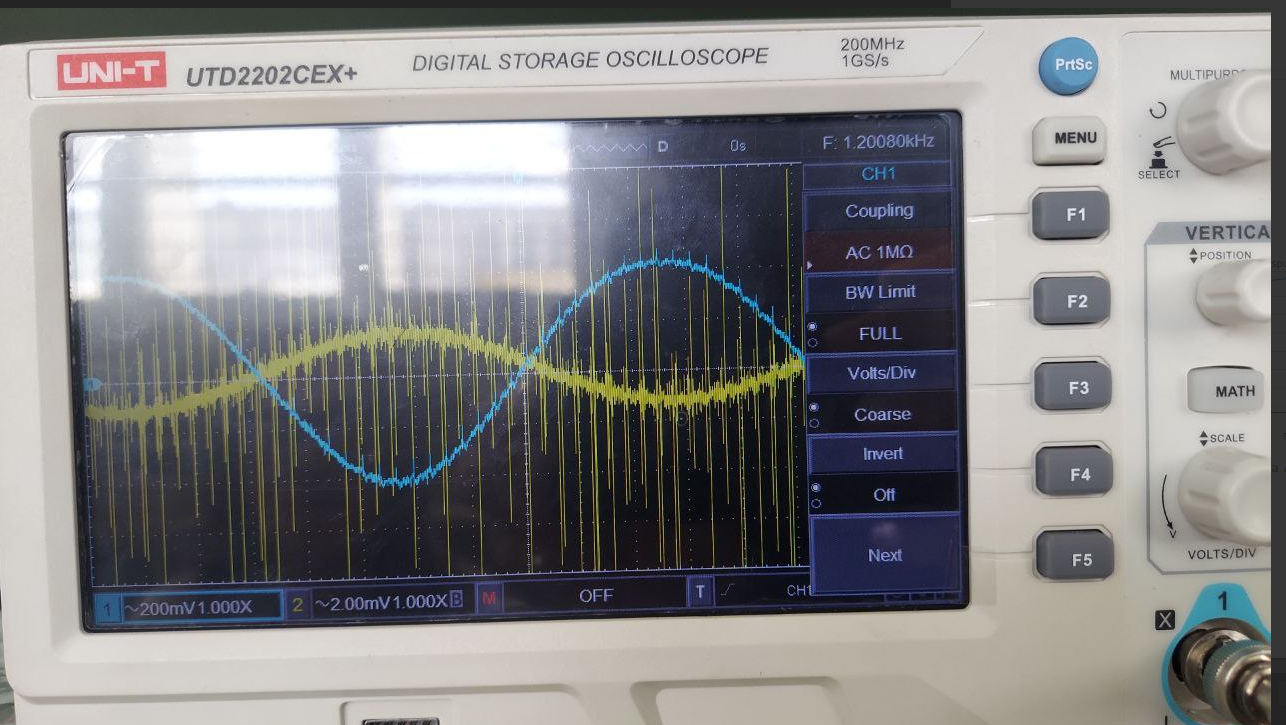
\includegraphics[width=0.8\textwidth]{src/images/resultados/p3/ganancia-etapa-impulsora.png}
    \caption{Ganancia etapa impulsora}
    \label{fig:ganancia-etapa-impulsora}
\end{figure}

\begin{figure}
    \centering
    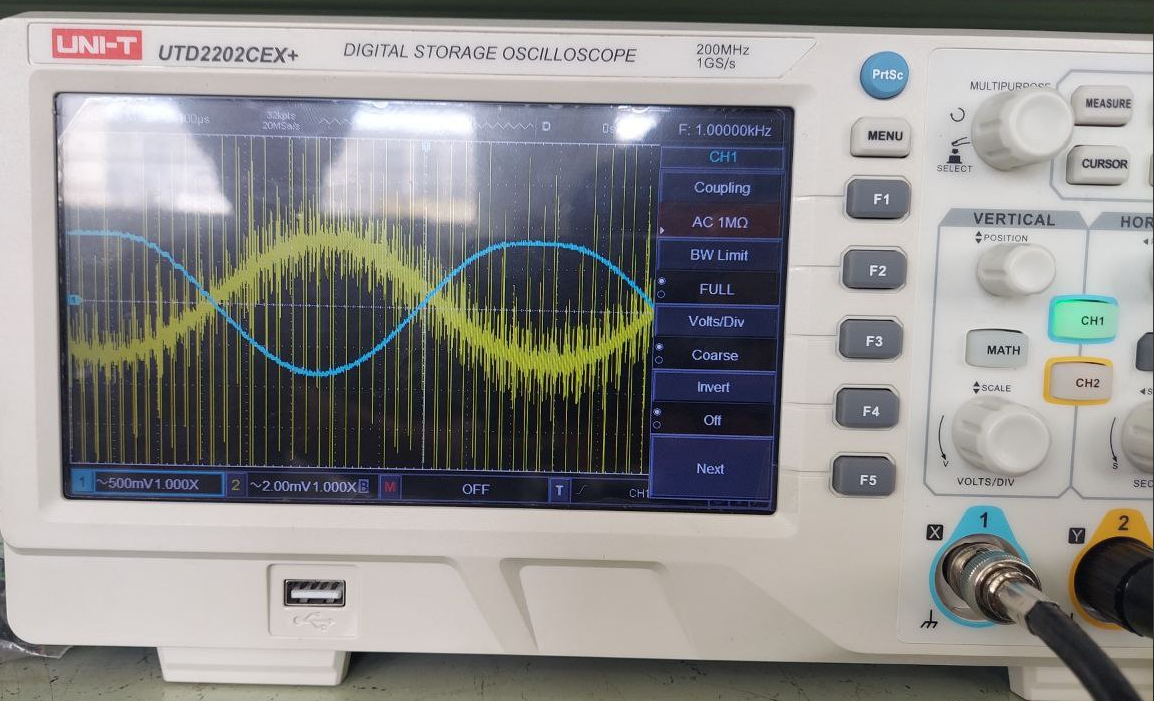
\includegraphics[width=0.8\textwidth]{src/images/resultados/p3/max-excursion-etapa-impulsora.png}
    \caption{Máxima excursión etapa impulsora}
    \label{fig:max-excursion-etapa-impulsora}
\end{figure}

\FloatBarrier
\subsubsection{Puntos de operación amplificador multietapas acoplado}

\begin{table}[h!]
\centering
\begin{tabular}{|c|c|c|c|c|c|c|c|c|c|}
\hline
\textbf{Transistor} & \textbf{\(Vc[V]\)} & \textbf{\(\varDelta Vc[V]\)} & \textbf{\(Vb[V]\)} & \textbf{\(\varDelta Vb[V]\)} & \textbf{\(Ve[V]\)} & \textbf{\(\varDelta Ve[V]\)} & \textbf{\(Re[\Omega]\)} & \textbf{\(\varDelta Re[\Omega]\)} \\ \hline
Q1 & 7.2 & 0.4 & -0.02 & 0.01 & -0.8 & 0.04 & 4700 & 235 \\ \hline
Q2 & 7.6 & 0.4 & -0.06 & 0.01 & -0.64 & 0.04 & 4700 & 235 \\ \hline
Q3 & 8 & 1 & 8 & 1 & 9 & 1 & 6800 & 340 \\ \hline
Q4 & 10 & 1 & 2 & 0.2 & 3.6 & 0.4 & 5000 & 500 \\ \hline
Q5 & 10 & 1 & 3.6 & 0.4 & 2.6 & 0.2 & 20 & 1 \\ \hline
Q6 & -10 & 1 & 2 & 0.2 & -2 & 0.2 & 20 & 1 \\ \hline
\end{tabular}
\caption{Mediciones de voltaje DC transistores en amplificador multietapas acoplado}
\label{tab:med-mediciones-voltaje-dc-transistores-amplificador-multietapas-acoplado}
\end{table}

\begin{table}[h!]
\centering
\begin{tabular}{|c|c|c|c|c|c|c|}
\hline
\textbf{Parámetro} & \textbf{Transistor} & \textbf{Valor Teórico} & \textbf{Medición} & \textbf{Incertidumbre} & \textbf{Error Absoluto} & \textbf{Error Relativo} \\ \hline
$I_{c}$ & Q1 & 0.00062 & 0.000595745 & 0.000231084 & 0.00002426 & 3.91\% \\ \hline
$I_{c}$ & Q2 & 0.00062 & 0.000510638 & 0.000230574 & 0.00010936 & 17.64\% \\ \hline
$I_{c}$ & Q3 & -0.00237 & -0.002647059 & 0.000246516 & 0.00027706 & 11.69\% \\ \hline
$I_{c}$ & Q4 & 3.02E-04 & 0.00032 & 9.49947E-05 & 0.00001764 & 5.83\% \\ \hline
$I_{c}$ & Q5 & 3.50E-04 & 0.23 & 0.018227726 & 0.22965000 & 65614.29\% \\ \hline
$I_{c}$ & Q6 & 3.50E-04 & 0.23 & 0.018227726 & 0.22965000 & 65614.29\% \\ \hline
$V_{ce}$ & Q1 & 7.79 & 8 & 0.401995025 & 0.21000000 & 2.70\% \\ \hline
$V_{ce}$ & Q2 & 7.79 & 8.24 & 0.401995025 & 0.45000000 & 5.78\% \\ \hline
$V_{ce}$ & Q3 & 2.27 & 1 & 1.414213562 & 1.27000000 & 55.95\% \\ \hline
$V_{ce}$ & Q4 & 1.24 & 6.4 & 1.077032961 & 5.16000000 & 416.13\% \\ \hline
$V_{ce}$ & Q5 & 9.99 & 7.4 & 1.019803903 & 2.59000000 & 25.93\% \\ \hline
$V_{ce}$ & Q6 & -9.99 & -8 & 1.019803903 & 1.99000000 & 19.92\% \\ \hline
\end{tabular}
\caption{Puntos estáticos de operación transistor multietapas acoplado}
\label{tab:med-puntos-estaticos-operacion-transistor-multietapas-acoplado}
\end{table}

\FloatBarrier
\subsubsection{modelo dinámico amplificador multietapas modo diferencial}

\begin{table}[h!]
\centering
\begin{tabular}{|c|c|c|c|c|c|}
\hline
\textbf{\(Vg[V]\)} & \textbf{\(\varDelta Vg[V]\)} & \textbf{\(Vi[V]\)} & \textbf{\(\varDelta Vi[V]\)} & \textbf{\(Rp[\Omega]\)} & \textbf{\(\varDelta Rp[\Omega]\)} \\ \hline
0.52 & 0.01 & 0.17 & 0.01 & 42000 & 4200 \\ \hline
\end{tabular}
\caption{Mediciones impedancias de entrada circuito multietapas modo diferencial}
\label{tab:med-impedancias-entrada-circuito-multietapas-modo-diferencial}
\end{table}

\begin{table}[h!]
\centering
\begin{tabular}{|c|c|c|c|c|c|}
\hline
\textbf{\(Vo_{sc}[V]\)} & \textbf{\(\varDelta Vo_{sc}[V]\)} & \textbf{\(Vo_{cc}[V]\)} & \textbf{\(\varDelta Vo_{cc}[V]\)} & \textbf{\(Rp[\Omega]\)} & \textbf{\(\varDelta Rp[\Omega]\)} \\ \hline
0.52 & 0.04 & 0.32 & 0.02 & 100 & 5 \\ \hline
\end{tabular}
\caption{Mediciones impedancia de salida amplifiador multietapa}
\label{tab:med-impedancia-salida-amplifiador-multietapa}
\end{table}

\begin{table}[h!]
\centering
\begin{tabular}{|c|c|c|c|}
\hline
\textbf{\(Vi[V]\)} & \textbf{\(\varDelta Vi[V]\)} & \textbf{\(Vo[V]\)} & \textbf{\(\varDelta Vo[V]\)} \\ \hline
0.0036 & 0.0002 & 0.52 & 0.04 \\ \hline
\end{tabular}
\caption{Ganancia amplificador multietapas modo diferencial}
\label{tab:med-ganancia-amplificador-multietapas-modo-diferencial}
\end{table}


\begin{table}[h!]
\centering
\begin{tabular}{|c|c|c|c|c|c|}
\hline
\textbf{Parámetro} & \textbf{Valor} & \textbf{Medición} & \textbf{Incertidumbre} & \textbf{Error Absoluto} & \textbf{Error Relativo} \\ \hline
$[Z] d$ & 43,990 & 20400 & 2771.263618 & 23590 & 53.63\% \\ \hline
$[Z] o$ & 132 & 62.5 & 16.40625 & 69.5 & 52.65\% \\ \hline
$[A]$ & 379.22 & 144.444444444444 & 13.70592797 & 234.7755556 & 61.91\% \\ \hline
\end{tabular}
\caption{Modelo dinámico amplificador multietapas modo diferencial}
\label{tab:med-modelo-dinamico-amplificador-multietapas-modo-diferencial}
\end{table}

\begin{figure}[ht]
    \centering
    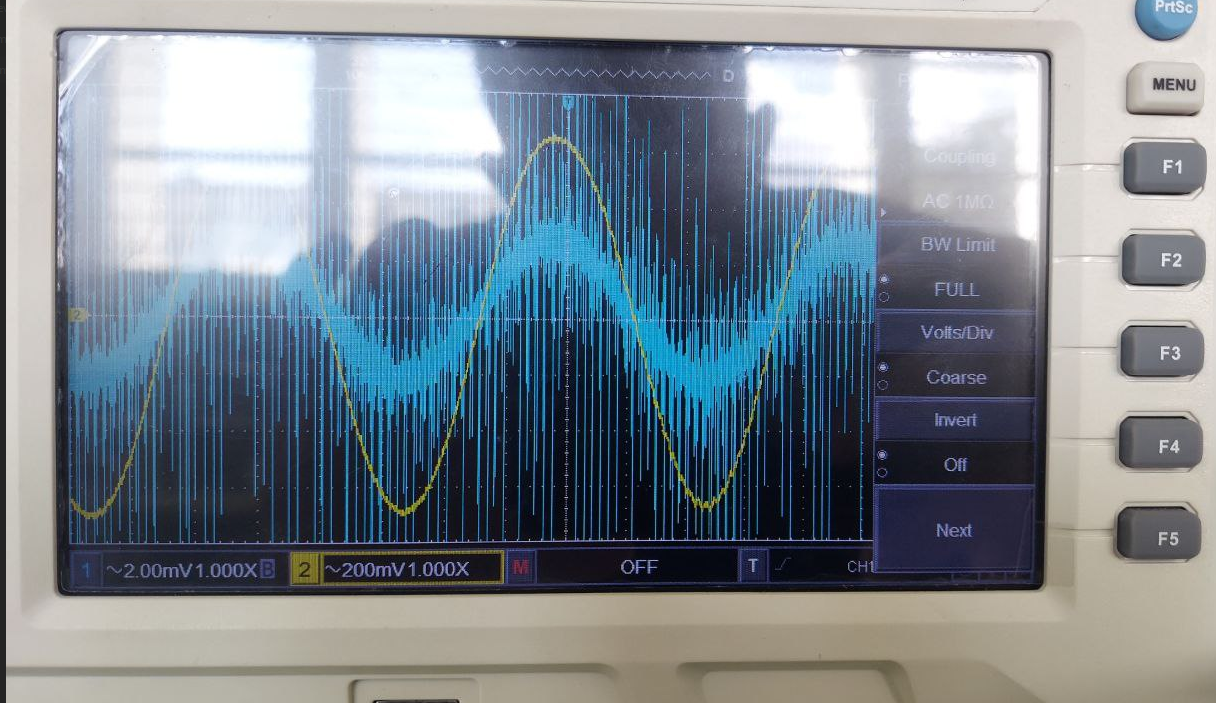
\includegraphics[width=0.8\textwidth]{src/images/resultados/p3/ganancia-multietapas-mod-diff.png}
    \caption{Ganancia del modelo dinámico amplificador multietapas modo diferencial}
    \label{fig:ganancia-multietapas-mod-diff}
\end{figure}

\begin{figure}[ht]
    \centering
    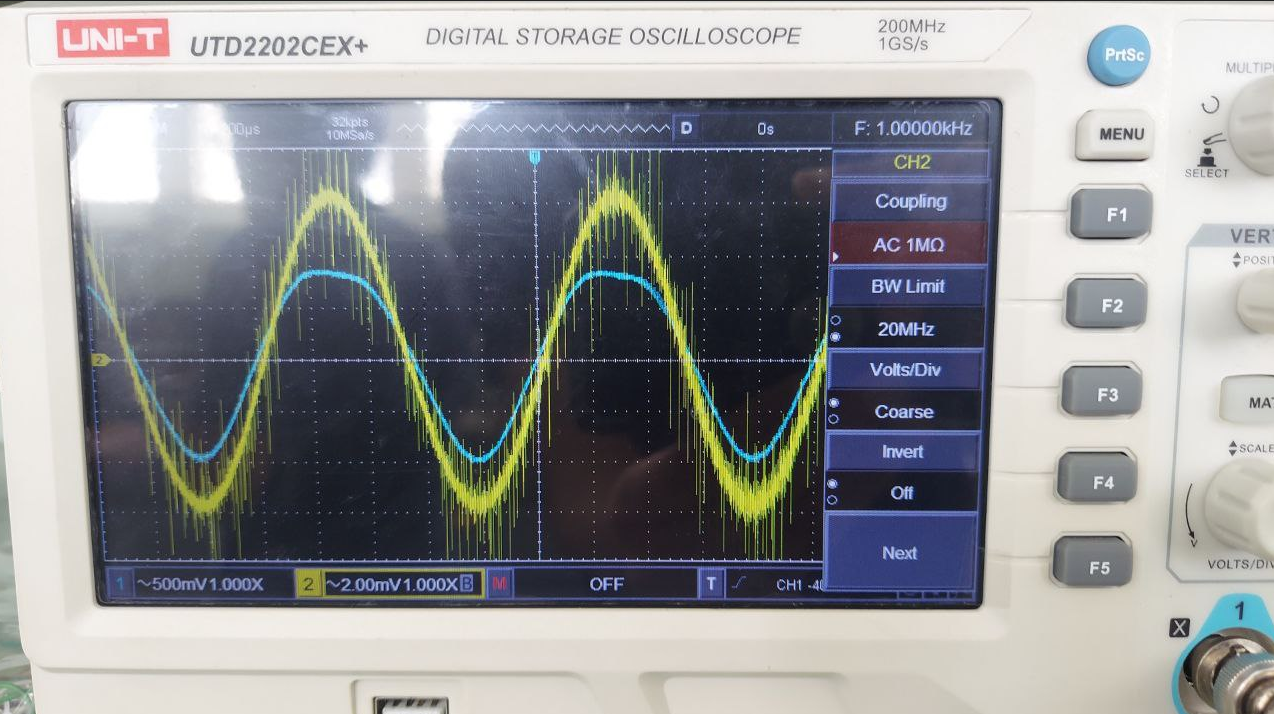
\includegraphics[width=0.8\textwidth]{src/images/resultados/p3/max-excursion-multietapas-mod-diff.png}
    \caption{Máxima excursión del modelo dinámico amplificador multietapas modo diferencial}
    \label{fig:med-max-excursion-multietapas-mod-diff}
\end{figure}

\FloatBarrier
\subsubsection{modelo dinámico amplificador multietapas modo común}

\begin{table}[h!]
\centering
\begin{tabular}{|c|c|c|c|c|c|}
\hline
\textbf{\(Vg[V]\)} & \textbf{\(\varDelta Vg[V]\)} & \textbf{\(Vi[V]\)} & \textbf{\(\varDelta Vi[V]\)} & \textbf{\(Rp[\Omega]\)} & \textbf{\(\varDelta Rp[\Omega]\)} \\ \hline
0.032 & 0.004 & 0.008 & 0.0004 & 20000 & 1000 \\ \hline
\end{tabular}
\caption{Impedancia de entrada amplificador multietapas modo común}
\label{tab:med-impedancia-entrada-amplificador-multietapas-modo-comun}
\end{table}


\begin{table}[h!]
\centering
\begin{tabular}{|c|c|c|c|}
\hline
\textbf{\(Vi[V]\)} & \textbf{\(\varDelta Vi[V]\)} & \textbf{\(Vo[V]\)} & \textbf{\(\varDelta Vo[V]\)} \\ \hline
0.024 & 0.002 & 0.38 & 0.02 \\ \hline
\end{tabular}
\caption{Ganancia amplificador multietapas modo común}
\label{tab:med-ganancia-amplificador-multietapas-modo-comun}
\end{table}

\begin{table}[h!]
\centering
\begin{tabular}{|c|c|c|c|c|c|}
\hline
\textbf{Parámetro} & \textbf{Valor} & \textbf{Medición} & \textbf{Incertidumbre} & \textbf{Error Absoluto} & \textbf{Error Relativo} \\ \hline
$[Z] d$ & 49000 & 41142.85714 & 5974.907966 & 7857.142857 & 16.03\% \\ \hline
$[Z] o$ & 132 & 62.5 & 602.0083575 & 69.5 & 52.65\% \\ \hline
$[A]$ & 40.05 & 15.83333333 & 1.560569795 & 24.21666667 & 60.47\% \\ \hline
\end{tabular}
\caption{Modelo dinámico amplificador multietapas modo común}
\label{tab:med-modelo-dinamico-amplificador-multietapas-modo-comun}
\end{table}

\begin{figure}
    \centering
    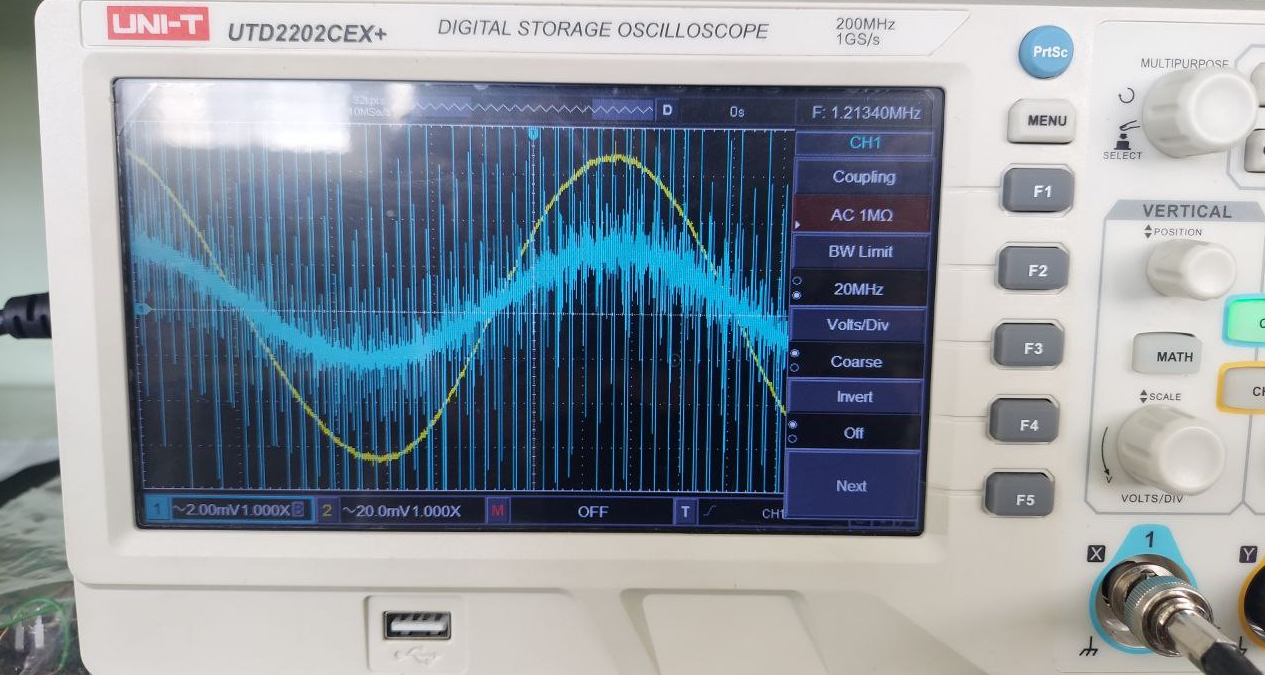
\includegraphics[width=0.8\textwidth]{src/images/resultados/p3/ganancia-multietapas-mod-comun.png}
    \caption{Ganancia del modelo dinámico amplificador multietapas modo común}
    \label{fig:ganancia-multietapas-mod-comun}
\end{figure}

\begin{figure}[ht]
    \centering
    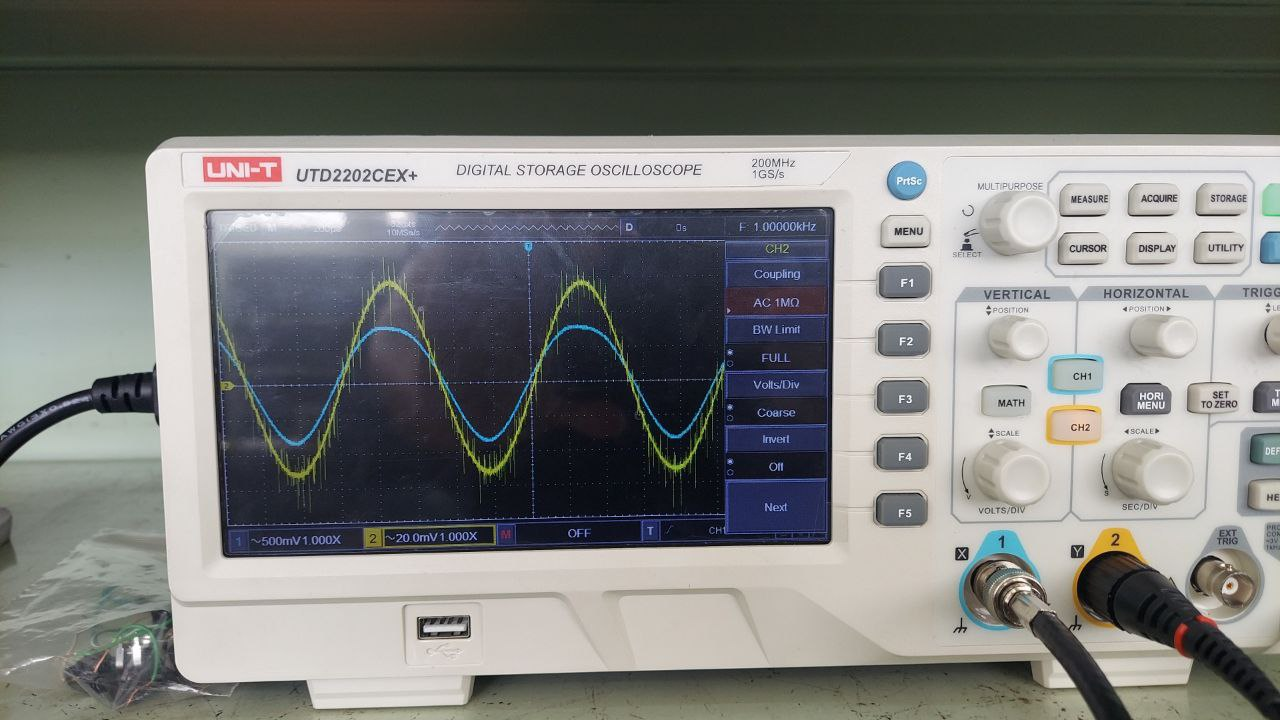
\includegraphics[width=0.8\textwidth]{src/images/resultados/p3/max-excursion-multietapas-mod-comun.png}
    \caption{Máxima excursión del modelo dinámico amplificador multietapas modo común}
    \label{fig:med-max-excursion-multietapas-mod-comun}
\end{figure}


\FloatBarrier
\subsection{Análisis respuesta en frecuencia}


\begin{itemize}
    \item Observando el punto estático de operación del cuadro \ref{tab:med-puntos-estaticos-operacion-amplificador-multietapa-respuesta-frecuencia} se observa que los corresponden a los teóricos exepto para los valores de corriente $I_c$ en la etapa de potencia, este error podría deberse a que no se usa la expresión corecta para hallar la medición indirecta correcta.
    \item En la figura \ref{fig:superposicion-respuesta-frecuencia-amplificador-multietapas-acoplado-condensadores} al superponer la respuesta en frecuencia medida con la simulación una correspondencia en la curva de la respuesta, tienen aproximadamente el mismo valor máximo y el mismo ancho de banda.
    \item En la figura \ref{fig:respuesta-frecuencia-amplificador-multietapas-acoplado-sin-condensadores} podemos observar que la respuesta en frecuencia al quitar los condensadores de acople cambia totalmente, teniendo una magnitud máxima de aproximadamente -20dB y cambiando totalmente el ancho de banda. Esto puede ser debido a una mala conexión del cable que sustituye al condensador de acople entre la etapa de potencia y la etapa de impulsora. Ya que dicho cable debería estar conectado al colector de $Q_3$ y al terminar la práctica se observó que estaba conectado al emisor.

\end{itemize}
\FloatBarrier
\subsection{Realimentación}
La ilustración \ref{ilus:amplificador-base} muestra el modelo dinámico del amplificador base. Cuyos parámetros son los mostrados en la tabla \ref{tab:amplificador-base-dinamico}.

\begin{ilustracion}[ht]
    \centering
    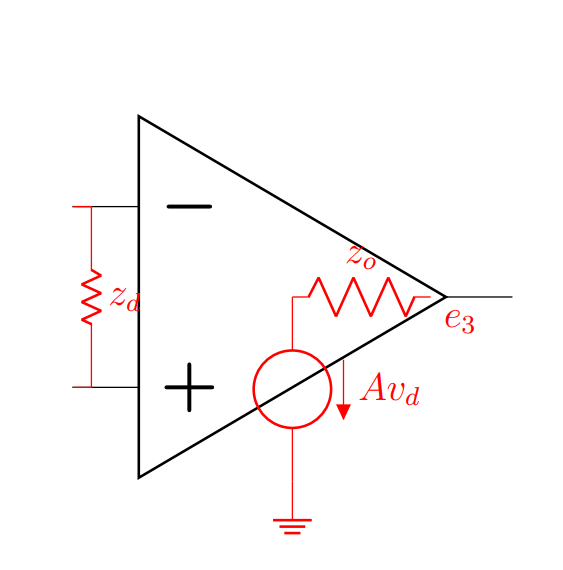
\includegraphics[width=0.6\textwidth]{src/images/p5/modelo-amplificador.png}
    \caption{Modelo dinámico del amplificador base}
    \label{ilus:amplificador-base}
\end{ilustracion}
Ahora calculamos los parámetros del amplificador realimentado negativamente.

para la impedancia de entrada $Z_i$ tenemos:

$$Z_i = R_s = 3.3 k\Omega$$

Y la impedancia de salida viene dada por la expresión:

$$Z_o = \frac{R_o}{A / (1 + \frac{R_f}{R_s})}$$

Por lo tanto el valor de $Z_o$ es:

$$Z_o = 0.137 \Omega$$

El valor de la ganancia de la realimentación negativa es: 

$$A_{fb} = - \frac{R_f}{R_s} = - \frac{11k\Omega}{3.3k\Omega} = -3.33$$

Y debido a que $A => \infty$ en el amplificador base, el valor de la ganancia de la realimentación negativa es:

$$A = -\frac{1}{\beta}$$

despejando $\beta$ de la expresión anterior, tenemos:

$$\beta = -\frac{1}{A} = -\frac{1}{3.33} = 0.333$$

Para encontrar las frecuencias de corte inferior utilizamos la expresión:

$$f_{Lf} = \frac{f_{Lb}}{1 + A_{b}}$$

entonces:

$$f_{Hf} = \frac{69.61 Hz}{1 + 49.54} = 1.37 Hz$$

Para hallar la frecuencia de corte superior utilizamos la expresión:

$$f_{Hf} = f_{Hb}\cdot (1 + A_{b})$$

Por lo tanto:

$$f_{Hf} = 11kHz\cdot (1 + 49.54) = 555.94KHz$$

\begin{table}[ht]
    \centering
    \begin{tabular}{|c|c|c|c|}
        \hline
        \textbf{Parámetro} & \textbf{Valor} \\ \hline
        $Z_i$ & $3.3$ [$k\Omega$] \\ \hline
        $Z_o$ & $0.17 $ [$\Omega$] \\ \hline
        $A_b$ & $-3.33$ \\ \hline
        $f_L$ & $1.37$ [$Hz$] \\ \hline
        $f_H$ & $555.94$ [$kHz$] \\ \hline
    \end{tabular}
    \caption{Valores de los parámetros dinámicos del amplificador Realimentado}
    \label{tab:amplificador-base-dinamico}

\end{table}

Ahora, para el amplificador realimentado positivamente, procedemos a calcular la ganancia:

$$A_{fb} = 1 + \frac{R_f}{R_s} = 1 + \frac{11k\Omega}{3.3k\Omega} = 4.33$$

La impedancia de entrada con realimentación positiva es:

$$ Z_i = \frac{Z_d \cdot A_b}{1 + \frac{R_f}{R_s}} = \frac{43.99k\Omega \cdot 300}{1 + \frac{11k\Omega}{3.3k\Omega}} = 3.05M\Omega$$

Y la impedancia de salida con realimentación positiva es igual a la impedancia de salida de realimentación negativa:

$$Z_o = 0.137 \Omega$$

La ilustración \ref{ilus:amplificador-realimentado-negativo} muestra el circuito del amplificador realimentado negativamente construido en multisim.

\begin{ilustracion}[ht]
    \centering
    \includegraphics[width=1.0\textwidth]{src/images/p5/Prelaboratorio 5 - Realimentación negativa - circuito.png}
    \caption{Circuito amplificador con realimentación negativa}
    \label{ilus:amplificador-realimentado-negativo}
\end{ilustracion}
\FloatBarrier

En la ilustración \ref{ilus:ganancia-realimentacion-negativa} podemos observar una ganancia de aproximadamente $3.3$ que coincide con la ganancia de los cálculos.

\begin{ilustracion}[ht]
    \centering
    \includegraphics[width=1\textwidth]{src/images/p5/Prelaboratorio 5 - Retroalimentación negativa - Ganancia.png}
    \caption{Ganancia de la realimentación negativa}
    \label{ilus:ganancia-realimentacion-negativa}
\end{ilustracion}

En la ilustración \ref{ilus:respuesta-frecuencia-realimentacion-negativa} podemos observar un aumento en el ancho de banda con realimentación negativa. Podemos observar que las frecuencias de corte coinciden con los cálculados previamente.

\begin{ilustracion}[ht]
    \centering
    \includegraphics[width=1.0\textwidth]{src/images/p5/Prelaboratorio 5 - retroalimentación negativa - respuesta en frecuencia.png}
    \caption{Respuesta en frecuencia del amplificador realimentado negativamente}
    \label{ilus:respuesta-frecuencia-realimentacion-negativa}
\end{ilustracion}
\FloatBarrier

% Realimentación positiva

La ilustración \ref{ilus:circuito-realimentacion-positiva-sin-condensador} muestra la construcción del circuito del amplificador realimentado positivamente.

\begin{ilustracion}[ht]
    \centering
    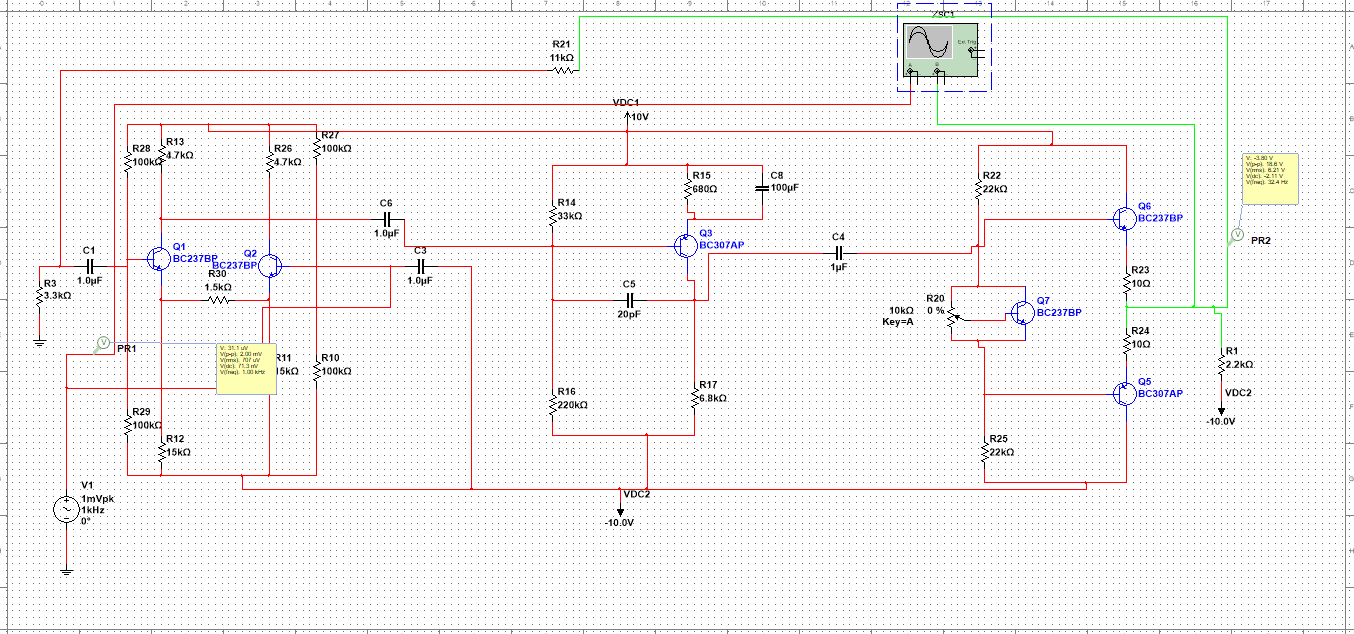
\includegraphics[width=\textwidth]{src/images/p5/Prelaboratorio 5 - Realimentacion positiva sin condensador - circuito.png}
    \caption{Circuito de realimentación positiva sin condensador}
    \label{ilus:circuito-realimentacion-positiva-sin-condensador}
\end{ilustracion}

La ganancia de este amplificador se puede observar en la ilustración del \ref{ilus:ganancia-circuito-realimentacion-positiva-sin-condensador} y podemos observar que coincide con la ganancia calculada anteriormente de 4.33. Sin embargo podemos observar que despues de un tiempo la ganancia cambia y toma la forma mostrada en la ilustración \ref{ilus:ganancia-circuito-realimentacion-positiva-sin-condensador-despues-de-unos-segundos}.

\begin{ilustracion}[ht]
    \centering
    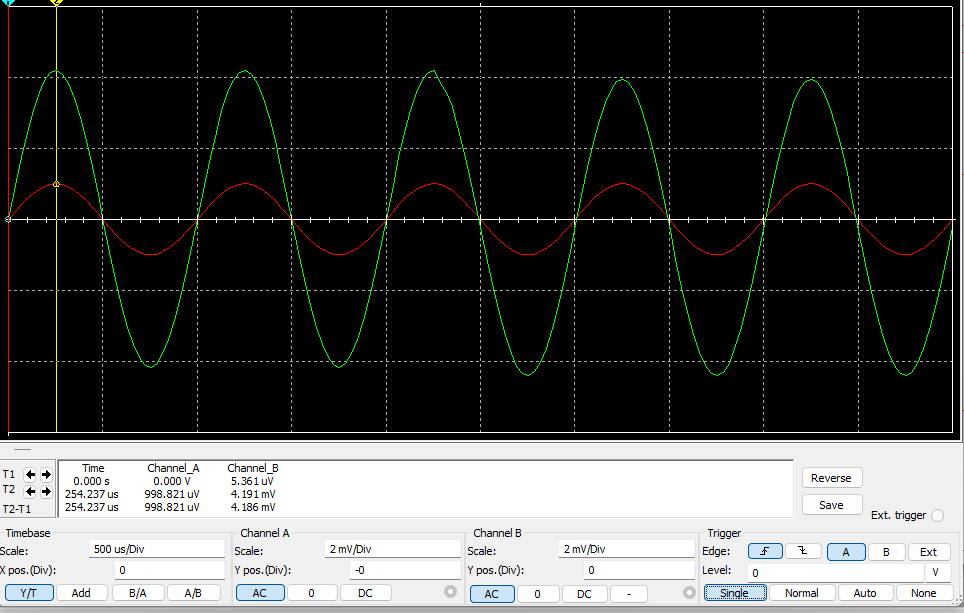
\includegraphics[width=\textwidth]{src/images/p5/Prelaboratorio 5 - Realimentacion positiva sin condensador - ganancia.png}
    \caption{Ganancia del circuito de realimentación positiva sin condensador}
    \label{ilus:ganancia-circuito-realimentacion-positiva-sin-condensador}
\end{ilustracion}
\FloatBarrier


\begin{ilustracion}[ht]
    \centering
    \includegraphics[width=\textwidth]{src/images/p5/Prelaboratorio 5 - Retroalimentación positiva sin condensador despues de unos segundos.png}
    \caption{Ganancia del circuito de realimentación positiva sin condensador despues de unos segundos}
    \label{ilus:ganancia-circuito-realimentacion-positiva-sin-condensador-despues-de-unos-segundos}
\end{ilustracion}
\FloatBarrier

Podemos observar la respuesta en frecuencia del amplificador realimentado positivamente en la ilustración \ref{ilus:respuesta-amplificador-realimentacion-positiva-sin-condensador}.

\begin{ilustracion}[ht]
    \centering
    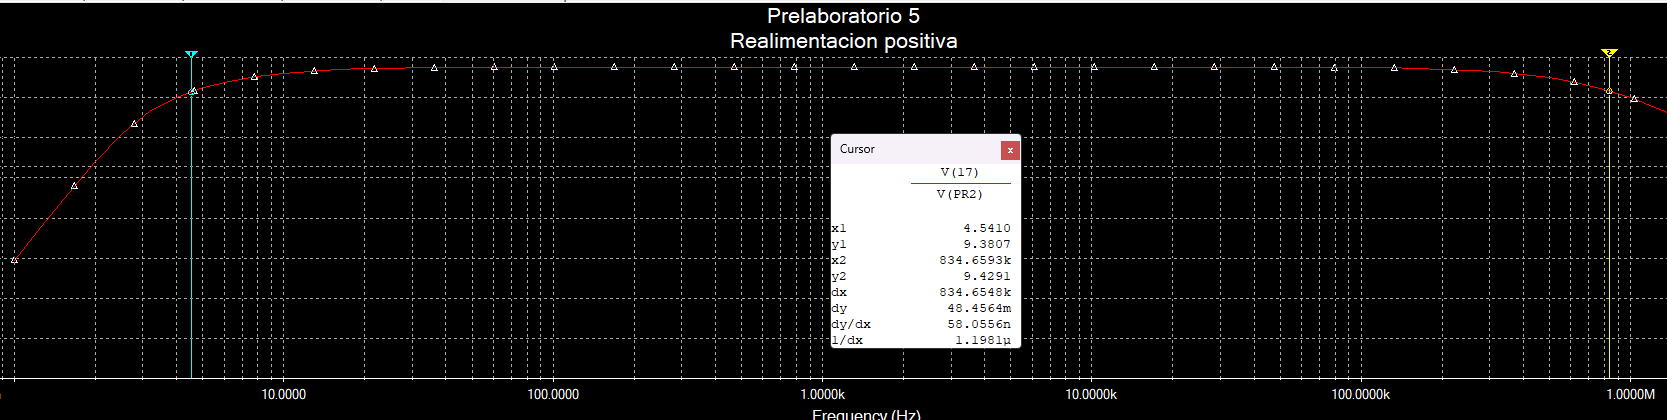
\includegraphics[width=\textwidth]{src/images/p5/Prelaboratorio 5 - realimentacion positiva sin condensador - respuesta en frecuencia.png}
    \caption{Respuesta en frecuencia del amplificador con Realimentación positiva sin condensador} 
    \label{ilus:respuesta-amplificador-realimentacion-positiva-sin-condensador}
\end{ilustracion}

Amplificador realimentado positiva y negativamente

La ilustración \ref{ilus:circuito-amplificador-realimentacion-positiva-y-negativa} muestra el circuito del amplificador con realimentación positiva y negativa con condensador.

\begin{ilustracion}[ht]
    \centering
    \includegraphics[width=\textwidth]{src/images/p5/prelaboratorio 5 - circuito realimentación positiva con condensador.png}
    \caption{Circuito con realimentación positiva y negativa} 
    \label{ilus:circuito-amplificador-realimentacion-positiva-y-negativa}
\end{ilustracion}
\FloatBarrier

La ganancia este amplificador se puede observar en la ilustración \ref{ilus:ganancia-amplificador-realimentacion-positiva-y-negativa}.
\begin{ilustracion}[ht]
    \centering
    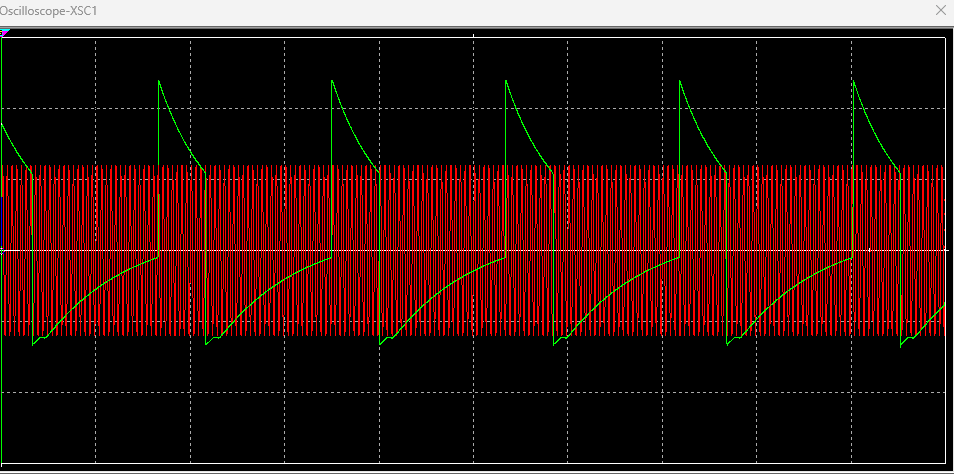
\includegraphics[width=\textwidth]{src/images/p5/Prelaboratorio 5 - Ganancia realimentacion positiva con condensador.png}
    \caption{Ganancia con realimentación positiva y negativa} 
    \label{ilus:ganancia-amplificador-realimentacion-positiva-y-negativa}
\end{ilustracion}
\FloatBarrier

La respuesta en frecuencia del amplificador se puede observar en la ilustración \ref{ilus:respuesta-amplificador-realimentacion-positiva-y-negativa}.

\begin{ilustracion}[ht]
    \centering
    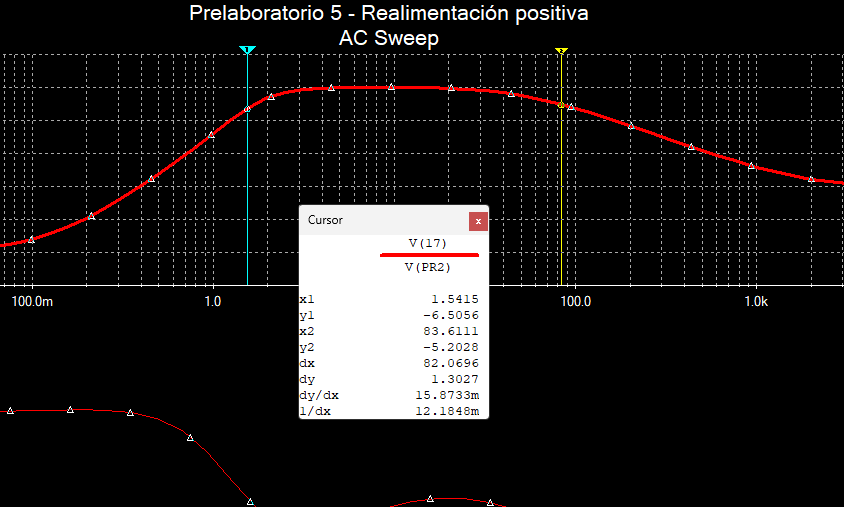
\includegraphics[width=\textwidth]{src/images/p5/Prelaboratorio 5 - Respuesta en frecuencia - realimentacion positiva con condensador.png}
    \caption{Circuito con realimentación positiva y negativa} 
    \label{ilus:respuesta-amplificador-realimentacion-positiva-y-negativa}
\end{ilustracion}

\FloatBarrier